\documentclass[11pt]{article}
\usepackage[margin=1in]{geometry}
\usepackage{amsmath,amsthm,amssymb}
\usepackage{enumitem, graphicx, float, caption}
\usepackage{amsmath}
\usepackage{bm}
\usepackage{parskip}
\usepackage{lipsum}
\usepackage{tikz}
\usepackage{listings}
\usepackage{xcolor}
\usepackage{float}
\usepackage{subcaption}
\usepackage{graphicx}
\usepackage[utf8]{inputenc}
\usetikzlibrary{arrows.meta}

\definecolor{codegreen}{rgb}{0,0.6,0}
\definecolor{codegray}{rgb}{0.5,0.5,0.5}
\definecolor{codepurple}{rgb}{0.58,0,0.82}
\definecolor{backcolour}{rgb}{0.95,0.95,0.92}

\lstdefinestyle{mystyle}{
    backgroundcolor=\color{backcolour},
    commentstyle=\color{codegreen},
    keywordstyle=\color{magenta},
    numberstyle=\tiny\color{codegray},
    stringstyle=\color{codepurple},
    basicstyle=\ttfamily\tiny,
    breakatwhitespace=false,
    breaklines=true,
    captionpos=b,
    keepspaces=true,
    numbers=left,
    numbersep=5pt,
    showspaces=false,
    showstringspaces=false,
    showtabs=false,
    tabsize=2
}

\lstset{xleftmargin=.020\textwidth, xrightmargin=.020\textwidth}

\setcounter{MaxMatrixCols}{26}
\setlength\parindent{0pt}
\counterwithin{equation}{enumi}


\begin{document}
    \noindent Nathan Burwig \\
    Math 87 HW  \\
    Due 
    
    \hrulefill

    \begin{center}
    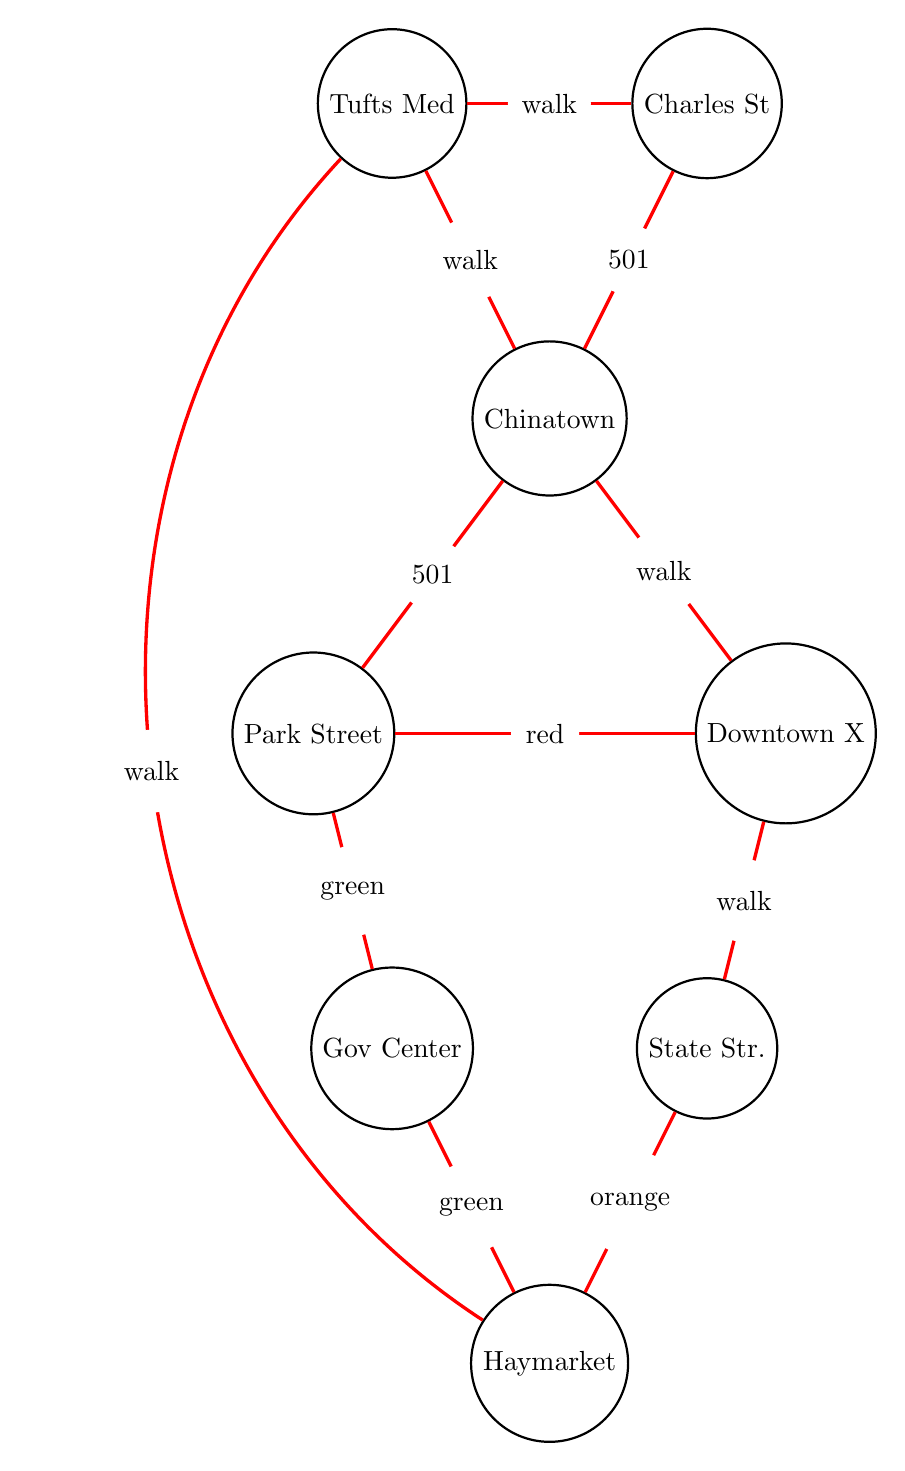
\begin{tikzpicture}
        \begin{scope}[every node/.style = {circle, thick, draw}]
            \node (H) at (0, 0)    {Haymarket};
            \node (G) at (-2, 4)   {Gov Center};
            \node (S) at (2, 4)    {State Str.};
            \node (D) at (3, 8)    {Downtown X};
            \node (P) at (-3, 8)   {Park Street};
            \node (C) at (0, 12)   {Chinatown};
            \node (T) at (-2, 16)  {Tufts Med};
            \node (L) at (2, 16)   {Charles St};
        \end{scope}

        \begin{scope}[>={Stealth[black]},
                every node/.style={fill=white,circle},
                every edge/.style={draw=red,very thick}]
                \path (L) edge node {walk} (T);
                \path (C) edge node {walk} (T);
                \path (L) edge node {501} (C);
                \path (C) edge node {501} (P);
                \path (C) edge node {walk} (D);
                \path (D) edge node {walk} (S);
                \path (P) edge node {red} (D);
                \path (P) edge node {green} (G);
                \path (G) edge node {green} (H);
                \path (S) edge node {orange} (H);
                \path (T) edge[bend right=50] node {walk} (H);

        \end{scope}
    \end{tikzpicture}
    \end{center}
    

\end{document}

